% Do NOT change this "Section" title
% and do NOT add more "Section" level titles.
\pagebreak
\section{Implementation}\label{sec:implementation}
As mentioned in Section~\ref{sec:introduction}, the Sensor Fusion is divided into two parts: Software architecture and Sensor fusion calculations. Sensor fusion calculations are in turn divided into attitude
calculations and dead reckoning.

\subsection{Software architecture}
To meet the software requirements it was decided to use Ada Tasks and Ada
Protected Objects. Protected objects are a special type of objects within Ada
to facilitate shared memory in a type safe way. A requirement from the
customer was the use of the Ada Ravenscar profile. This profile limits
the use of tasks to make the program easier to verify and validate. This meant
that each protected object in use was only allowed to be called from no more than two
different tasks.

The common data structure within the Naiad AUV is the CAN message structure,
it has a message ID and payload. These messages were modelled as objects within
the Sensor fusion code and the CAN message type is the only data type that
is passed around between Ada Tasks.

To manage the incoming and outgoing data two tasks were set up for each link,
TCP\_IN and TCP\_OUT for the ethernet connection as well as CAN\_IN and CAN\_OUT for
the CAN bus connection. Each one of these tasks had only one responsibility, which
was to either send or receive CAN messages.
The next task to be added was the Main
task which would do all the calculations. The design in this stage had five
different tasks with distinct responsibility, though one main problem left to solve
was the requirement that in this design the Main task would have to do a lot of
filtering of CAN messages both to and from the TCP and CAN connection. To solve this
two new tasks were introduced, the TCP\_IN\_FILTER and CAN\_IN\_FILTER. The filtering
tasks would be given a set of CAN message IDs on boot up that were of interest to
the Main task. The Main task had now only one responsibility left and that was
to do the actual sensor fusion calculations.

\begin{figure}[ht]
    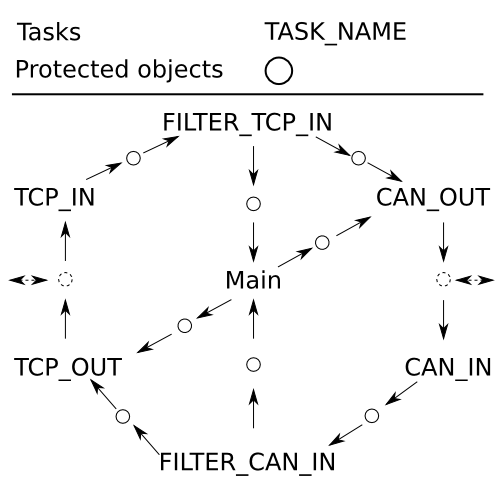
\includegraphics[width=0.5\textwidth]{./figure/software_architecture.png}
    \caption{Sensor fusion software architecture. Showing the different tasks and
    how they interact with each other through several different protected objects.}
    \label{fig:software_architecture}
\end{figure}

The final design of the software architecture is seen in Figure \ref{fig:software_architecture}.
The dashed circles on the left and right side are protected objects specific for
the different hardware resources. For the CAN bus this is required because one
cannot read and write at the same time, but for the TCP connection multiple connections
can be done in parallel so this can be changed.


% You can use how many "subsections" and "subsubsections" you like.
\subsection{Sensor fusion calculations}
The Sensor fusion calculations consist of two parts, attitude calculations and
dead reckoning.

\subsection{Attitude Calculations}
The Vectornav VN100 IMU (Inertial Measurement Unit)~\cite{web:vn100} used in 
the Naiad AUV gets the yaw, pitch and roll values by integrating over the
angular velocities. However even when the IMU is kept still it still has
some residual angular velocities which causes the yaw, pitch and roll to drift
over time and hence need to be corrected.
The IMU corrects its roll and pitch values using its accelerometer 
readings which give the direction of gravity.
Once roll and pitch are corrected, the magnetometer reading is used to correct
the yaw value.

The Vectornav VN100 IMU has a Kalman
filter implemented which provides us with the compensated yaw, pitch and roll
values. However according to the requirements the magnetic fields cannot be
trusted in some competitions. This leads to the yaw values being unreliable.
Thus to correct yaw, a Fiber Optic Gyroscope (FOG)~\cite{web:fog1} is used.

A fiber optic gyroscope uses a laser interferometer to calculate the angular
speed of the gyroscope. The challenge is to
integrate the readings obtained from the FOG to the readings obtained from
the IMU. If one integrates the angular velocity from FOG one can get the yaw value, 
this value tells the angle the AUV rotates in the z axis attached to the AUV.
The idea is that this is the yaw angle that should be applied to the AUV after
the roll and pitch is done, that is the yaw should be the last operation to
reach from one state to other.

The IMU can output the yaw, pitch and roll in body frame of reference.
To use the FOG value it should be converted to roll, pitch and yaw order.
After that the yaw value of IMU can be replaced with the yaw from the FOG.
The following two methods were proposed to change the angle order from yaw,
pitch and roll to roll, pitch and yaw:
\begin{enumerate}
\item The idea is that for small changes in yaw, pitch and roll angles,
    the order in which the rotations are applied does not matter upto first
    degree of accuracy. So changes to yaw pitch and roll are calculated for
    IMU and the yaw change for FOG at each time step. If it is assumed that
    the AUV moves slowly and that the samples are taken fast enough, the changes
    to the angles will be small. Thus the rotation matrix from the previous
    step is multiplied with the rotation matrix obtained by combining the yaw
    from FOG and roll and pitch from IMU to get a new rotation matrix.
\item VN100 IMU can also output the Directional Cosine Matrix (DCM). The other method is to
    get the DCM and compare it to the rotation matrix obtained by
    applying rotations in roll, pitch and yaw order. Then one can derive
    formulas for the roll, pitch and yaw in terms of DCM matrix elements.
\end{enumerate}

\subsection{Dead Reckoning}
Dead reckoning is the name of the method used to calculate the x, y and z
coordinates of the AUV with the starting position as the origin.
The simplest way to do this is to integrate the accelerometer values
twice to get the position. However this can lead to large amounts of errors
because a small error in accelerometer increases exponentially with
time as it is multiplied with time squared. To avoid this the plan was
to use front and down facing cameras, which have stereo vision, and
calculate the velocity of the AUV. Then the velocity and acceleration
can be combined using Kalman filter to get a better estimate of the position.
